\documentclass[a4paper,fleqn]{cas-sc}

\usepackage[numbers]{natbib}
%\usepackage[authoryear]{natbib}
% \usepackage[authoryear,longnamesfirst]{natbib}
\usepackage{url}
\usepackage{float}
\usepackage{amssymb}  
\usepackage{booktabs} 
\usepackage{tabularx}
\newcolumntype{L}{>{\raggedright\arraybackslash}X}
\usepackage{graphicx}
\usepackage{amsthm}

\def\tsc#1{\csdef{#1}{\textsc{\lowercase{#1}}\xspace}}
\tsc{WGM}
\tsc{QE}
\tsc{EP}
\tsc{PMS}
\tsc{BEC}
\tsc{DE}

\begin{document}
\let\WriteBookmarks\relax
\def\floatpagepagefraction{1}
\def\textpagefraction{.001}
\newtheorem{remark}{Remark}

% Short title
\shorttitle{Incremental Verification Framework of LwM2M}

% Short author
% \shortauthors{Sini Chen et~al.}

% Main title of the paper
\title [mode = title]{Incremental Verification Framework of LwM2M for Shopfloor Operations with UPPAAL}                      


% \author[1]{Sini Chen}[orcid=0000-0003-3923-7972]
% \author[2]{Ran Li}[orcid=0000-0002-3492-1591]
% \author[1]{Zihan Tang}[orcid=]
% \author[1]{Huibiao Zhu}[orcid=0000-0002-0214-8565]

% \cormark[1]
% \ead{hbzhu@sei.ecnu.edu.cn}


% % Address/affiliation
% \affiliation[1]{organization={East China Normal University},
%     city={Shanghai},
%     postcode={20000}, 
%     country={China}}

% \affiliation[2]{organization={Nanjing University of Information Science and Technology},
%     % addressline={}, 
%     city={Nanjing},
%     postcode={695014}, 
%     country={China}}
    
% % Corresponding author text
% \cortext[cor1]{Corresponding author}



% Here goes the abstract
\begin{abstract}
The Lightweight Machine-to-Machine (LwM2M) protocol is a mainstream standard for device management and telemetry in constrained industrial IoT networks. However, its correctness, security, and performance under realistic conditions have not been jointly analyzed using formal methods. 

This paper presents an incremental formal modeling and verification framework for LwM2M tailored to Industry 4.0 scenarios with three layers. 
In the functional layer, we build deterministic timed automata in UPPAAL for the Bootstrap, Registration, and Observation interfaces, verifying reachability, mutual exclusion, and deadlock freedom. In the security layer, we extend the models with attacker automata capturing man‑in‑the‑middle, fake bootstrap server, replay, denial‑of‑service, and notification tampering. Verification confirms that all modeled attacks are feasible, exposing the lack of integrity and freshness protection. In the stochastic performance layer, we use UPPAAL Statistical Model Checking (SMC) to introduce packet loss, CoAP‑style retransmissions, and DTLS/OSCORE delays. Results show that security mechanisms incur a moderate throughput penalty, but when combined with retransmissions the system achieves near‑perfect reliability. Trace inclusion relations between layers enable reuse of functional properties, reducing verification effort. This work offers a unified formal treatment of LwM2M across functional, security, and performance dimensions using a single tool chain.
\end{abstract}

% Keywords
% Each keyword is seperated by \sep
\begin{keywords}
LwM2M\sep Formal verification\sep Statistical model checking\sep Industrial IoT
\end{keywords}

\maketitle

\section{Introduction}
The Internet of Things (IoT) has revolutionized industrial manufacturing, enabling real-time monitoring, remote configuration, and data-driven decision making \cite{malik2021industrial}. In such environments, the Lightweight Machine-to-Machine (LwM2M) protocol, defined by the Open Mobile Alliance (OMA), has emerged as a mainstream standard for device management and telemetry in constrained networks \cite{robles2024industrial}. LwM2M operates over CoAP and provides four core interfaces: Bootstrap, Registration, Device Management and Service Enablement, and Information Reporting \cite{jimenez2024managing}. In an Industry 4.0 scenario, a Manufacturing Execution System (MES) can act as the LwM2M Server, while shop‑floor devices such as sensors, actuators, and controllers can serve as LwM2M Clients. The correct functioning of these interfaces is critical for system reliability, security, and performance.

Despite its widespread adoption, the formal analysis of LwM2M has received limited attention. Existing work has explored various aspects: some studies focus on performance evaluation and protocol comparison under different network conditions \cite{parmigiani2021comparison}; others investigate security enhancements, such as integrating blockchain for auditability \cite{martin2020providing} or extending client-to-client communication with security mechanisms \cite{lanzieri2022secure}. Formal approaches have also been applied, including the use of Event-B for client implementation correctness \cite{mouakher2020toward} and model checking for the registration phase in isolation \cite{penchevaformal}. 
However, existing work remains fragmented: these efforts are often limited to specific interfaces, quality attributes, or execution settings, and rarely consider their interplay. Consequently, the joint interaction among functionality, security, and stochastic network behavior remains insufficiently understood.
Traditional testing methods are insufficient to uncover subtle logic flaws or to quantify the impact of network unreliability. Formal methods, particularly model checking, offer a rigorous alternative by enabling exhaustive exploration of system states \cite{woodcock2009formal}. Nevertheless, applying model checking to LwM2M is non‑trivial due to the combinatorial explosion of possible system states, which makes exhaustive verification extremely resource‑intensive. This problem is exacerbated by the addition of attacker automata and probabilistic and timed behavior.

In this paper, we present an incremental three‑layer formal modeling and verification framework for LwM2M tailored to industrial IoT scenarios. As illustrated in Fig.~\ref{roadmap}, the framework decomposes the analysis into three complementary dimensions, including \textbf{functional correctness}, \textbf{security resilience}, and \textbf{stochastic performance}. For each layer we construct formal models using UPPAAL and UPPAAL SMC, enabling a unified tool chain across all three dimensions.  The layers are designed to support trace inclusion – functional properties verified on the base model are inherited by the extended layers, reducing redundant verification.  Our contributions are as follows.

\begin{itemize}
    \item Functional Model (Layer I): We build deterministic timed automata in UPPAAL for the Bootstrap, Registration, and Observation interfaces, preserving all essential protocol states while abstracting away implementation details that do not affect logical correctness. We verify key functional properties such as reachability, mutual exclusion, and deadlock freedom. This functional model serves as a solid baseline for further analysis, and its correctness is reused in subsequent layers via trace inclusion.
    \item Security Model (Layer II): We extend the functional model with dedicated attacker automata to capture realistic threats. For each interface, we model multiple attack types: man‑in‑the‑middle, eavesdropping, fake bootstrap server, replay, denial‑of‑service, and notification tampering. Using UPPAAL, we verify that these attacks can indeed be carried out, exposing fundamental vulnerabilities such as lack of message integrity, server authentication, and freshness protection.
    \item Stochastic Performance Model (Layer III): We augment the models with probabilistic elements using UPPAAL Statistical Model Checking (SMC). We introduce packet loss ($0.5\%$), CoAP‑style retransmissions (max 4 times, exponential backoff), and security overhead delays (DTLS/OSCORE) based on empirical measurements and standard CoAP retransmission settings. We then evaluate the performance of three configurations: no security, security only, and security with retransmission. The results quantify the trade‑off between security and reliability, showing that retransmission can compensate for packet loss and restore near‑perfect reliability with acceptable overhead.
\end{itemize}

All models are implemented in UPPAAL, and the verification scripts are made available as supplementary material to ensure reproducibility. This work offers a unified formal treatment of LwM2M across functional, security, and performance dimensions using a single tool chain, which, to the best of our knowledge, has not been systematically explored before.

\begin{figure}[pos=htbp]
	\centering
	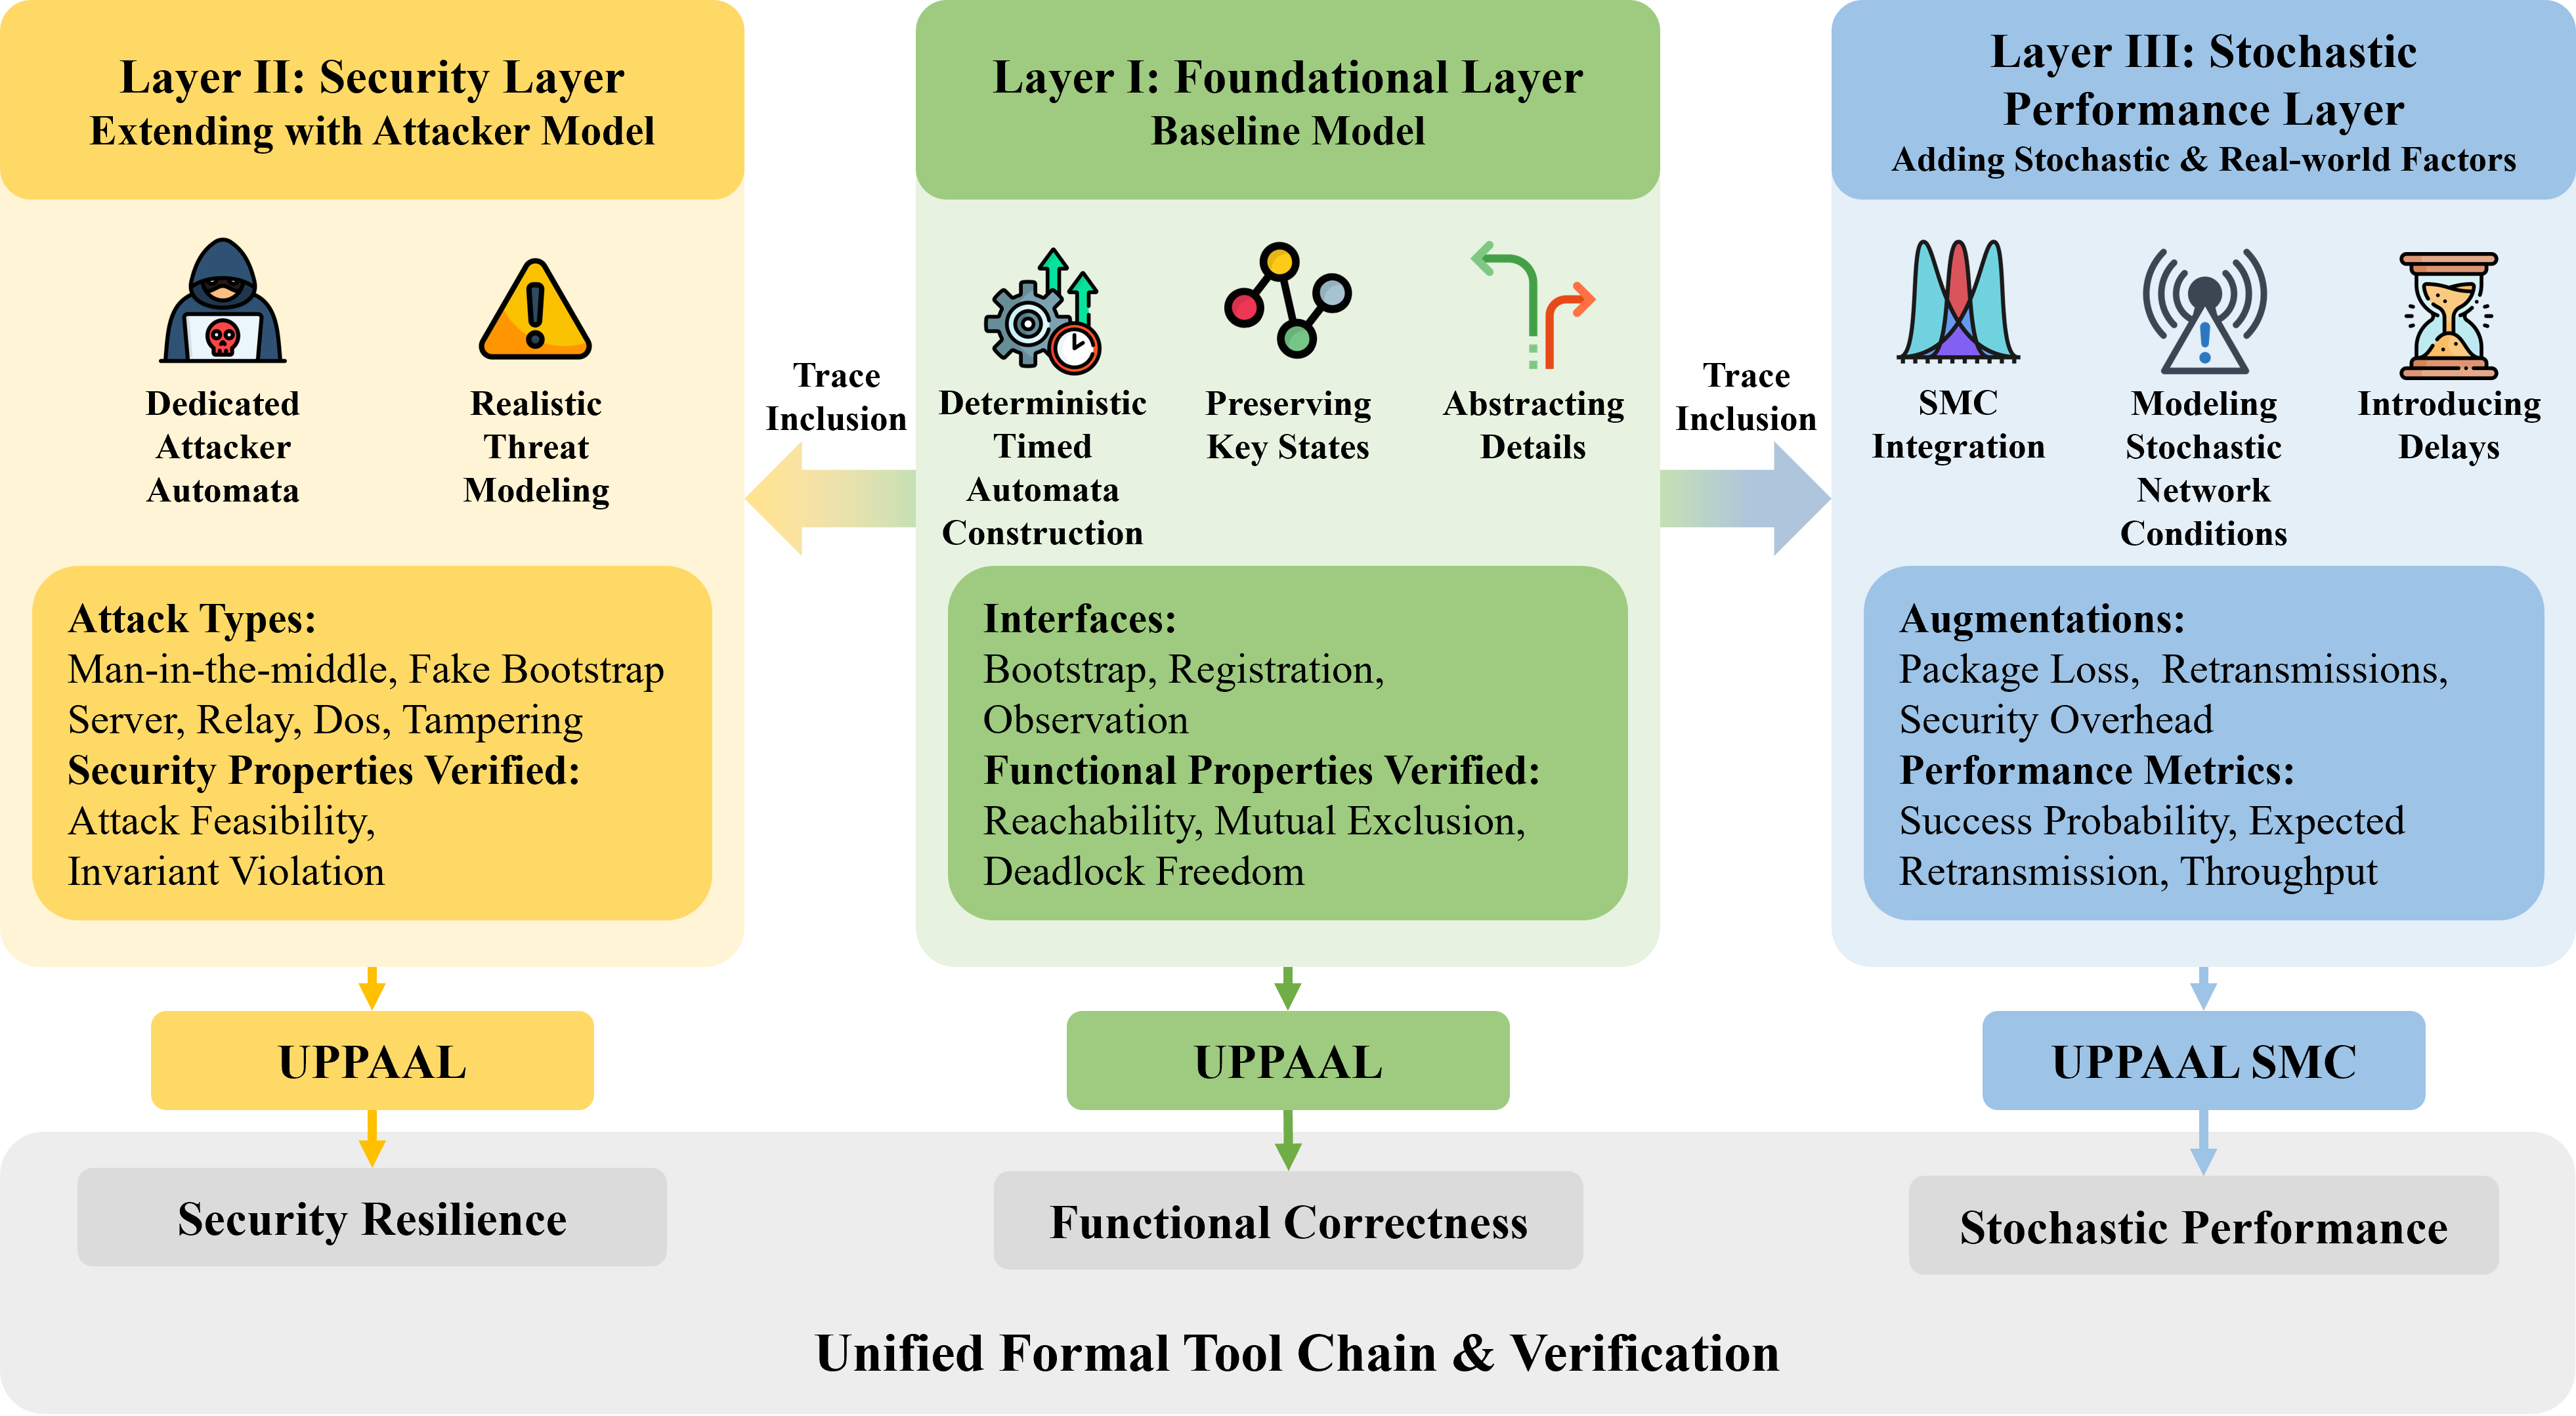
\includegraphics[width=0.9\textwidth]{figs/roadmap.png}
	\caption{Overview of the three‑layer formal verification framework for LwM2M.}
	\label{roadmap}
\end{figure}

The remainder of this paper is organized as follows. Section 2 provides background on LwM2M and UPPAAL/UPPAAL SMC, and discusses related work. Section 3 presents the functional model and its verification. Section 4 describes the security model, including the attacker automata and the verification results. Section 5 introduces the stochastic performance model and the experimental evaluation. Section 6 discusses the validity of our abstractions and the implications of the results. Finally, Section 7 concludes the paper and outlines future directions.

\section{Background}
This section introduces the essential concepts and related work that underpin our work. We first give an overview of the LwM2M protocol. Next, we briefly describe UPPAAL and UPPAAL SMC, the tools used for deterministic and probabilistic verification. Finally, we review existing studies on formal verification of IoT protocols, highlighting the gap that our work addresses.
\subsection{LwM2M Protocol Overview}
Lightweight Machine to Machine (LwM2M) is an open standard defined by the Open Mobile Alliance (OMA) for device management and telemetry in constrained Internet of Things (IoT) networks~\cite{alliance2017lightweight}. It builds on the Constrained Application Protocol (CoAP) and provides a compact, efficient architecture that enables remote management of resource-constrained devices~\cite{rao2015implementing}. The LwM2M ecosystem consists of three main logical entities: the \textit{LwM2M Client} (typically a sensor or actuator), the \textit{LwM2M Server} (a management platform, e.g., a Manufacturing Execution System), and the \textit{LwM2M Bootstrap Server} that initializes devices with security credentials and server configuration.

The protocol defines four core interfaces:
\begin{itemize}
\item \textbf{Bootstrap}: establishes initial security credentials and server information on the client.
\item \textbf{Registration}: allows the client to announce its presence and object capabilities to the server.
\item \textbf{Device Management \& Service Enablement}: provides operations such as read, write, execute, and create on device resources.
\item \textbf{Information Reporting}: enables the server to observe resource changes and receive asynchronous notifications.
\end{itemize}

In this work we focus on the Bootstrap, Registration, and Observation (information reporting) interfaces, because they capture the core lifecycle of device onboarding, server association, and runtime telemetry, which are the most critical interactions in the industrial shop‑floor scenario considered.

\subsection{UPPAAL and UPPAAL SMC}
UPPAAL is an integrated tool environment for modeling, simulation, and verification of real‑time systems modeled as networks of timed automata~\cite{larsen1997uppaal}. A timed automaton is a finite state machine extended with real‑valued clocks. In UPPAAL, a system is composed of several such automata running in parallel, communicating through channels and shared variables.

An automaton consists of a set of locations and edges. Locations can be ordinary, urgent (time cannot pass while in that location), or committed (the system cannot delay and must take an outgoing edge from a committed location immediately). Each edge is labeled with a guard (a clock constraint that must hold for the edge to be taken), a synchronization (either sending \texttt{c!} or receiving \texttt{c?} on a channel \texttt{c}), and an update (a sequence of assignments). Clocks are reset on edges as part of the update.

Properties are expressed in a subset of Timed Computation Tree Logic (TCTL). The most common formulas are: 
\begin{itemize}
    \item \texttt{E<> p}: there exists a path that eventually reaches a state satisfying p (reachability).
    \item \texttt{A[] p}: on all paths, p always holds (invariant).
    \item \texttt{A<> p}: on all paths, p is eventually reached (liveness).
\end{itemize}

UPPAAL verifies these properties exhaustively by exploring the entire state space.

When the model includes stochastic behavior (e.g., random delays, probabilistic branching), the exhaustive state‑space exploration becomes infeasible. UPPAAL SMC addresses this by performing a fixed number of stochastic simulations and using statistical inference to estimate the probability that a property holds within a given time bound~\cite{david2015uppaal}. Instead of TCTL, SMC uses queries of the form:
\begin{itemize}
    \item \texttt{Pr[<=T] (<> p)}: the probability that p is eventually reached within time T.
    \item \texttt{E[<=T] (max: expr)}: the expected maximum value of expr over simulations.
    \item \texttt{N[<=T] \{ expr1, expr2 \}}: generates N simulation traces for visual inspection.
\end{itemize}

All models presented in this work are implemented in UPPAAL, and the verification queries use the above syntax. The tool’s ability to combine deterministic and probabilistic modeling makes it particularly suitable for our three‑layer approach.

\subsection{Related Work}
\subsubsection{Formal Verification of IoT Protocols}
Formal methods have been widely applied to verify the correctness of IoT protocols. A variety of tools and modeling paradigms have been used. For instance, the functional correctness of RabbitMQ has been verified using timed automata in UPPAAL~\cite{DBLP:conf/trustcom/LiYZ20}. The Enhanced Group Communication CoAP protocol was modeled and verified using CSP~\cite{DBLP:journals/ijseke/ChenLZ24}. High‑level Petri nets have been employed to control IoT device behavior~\cite{DASILVAFONSECA20231462}. These studies demonstrate the maturity of formal techniques in this domain, yet they typically focus on a single aspect—most often functional correctness—in isolation.

Several efforts have attempted to combine functional and performance aspects. The MQTT protocol was formally specified and evaluated using both UPPAAL (for functional verification) and UPPAAL SMC (for performance analysis)~\cite{houimli2017formal}. Another study proposes formal models for verification, performance evaluation, and comparison of IoT communication protocols using CTL~\cite{hafaiedh2022formal}. These works demonstrate the feasibility of integrating functional and performance analyses within a single framework. However, security threats are not considered alongside these dimensions, leaving the interplay between security mechanisms and system reliability unexplored.

A recurring challenge in these works is state space explosion, which can hinder exhaustive verification. A systematic review on IoT capabilities composition identifies three main mitigation strategies: model simplification, model decomposition, and resource management~\cite{halba2023iot}. The decomposition strategy, in particular, aligns with our approach: we split the LwM2M protocol into three progressively incremental layers (functional, security, performance) and further decompose each layer into separate interface‑specific models. This modular design not only curbs state explosion but also enables reuse of verified components across layers.

To the best of our knowledge, no existing work provides a unified formal framework that integrates functional correctness, security attack modeling, and probabilistic performance evaluation for the LwM2M protocol. Our three‑layer approach fills this gap by building on the strengths of prior verification efforts while introducing novel elements—explicit attacker automata for security threats and probabilistic extensions for performance assessment—all within a single tool chain (UPPAAL / UPPAAL SMC).

\subsubsection{Security Analysis in Industrial IoT}
Ensuring the security of industrial IoT (IIoT) systems has attracted significant research interest, with proposals ranging from non‑formal approaches to fully formal verification.

Several techniques have been developed to assess vulnerabilities and enforce trust in IIoT environments without relying on exhaustive state‑space exploration. For instance, graph‑based frameworks have been used to model attack paths and evaluate vulnerability exploitability ~\cite{george2018graph}. Trust evaluation frameworks combine behavioral monitoring with reputation scores to detect malicious devices~\cite{wang2022toward}. Machine learning approaches, such as ensemble learning, have been applied to build intrusion detection models tailored to IIoT traffic~\cite{mohy2023ensemble}. Fuzzy logic has also been employed to assess information security risks in industrial networks~\cite{kerimkhulle2023fuzzy}. While these methods can provide practical security monitoring, they typically depend on heuristics, statistical thresholds, or expert knowledge. Consequently, they do not guarantee coverage of all possible attack sequences, nor do they offer a way to quantitatively compare the impact of different security mechanisms under varying network conditions.

In contrast, formal methods provide mathematical guarantees for IIoT protocols as well as IIoT systems. For CoAP, model checking has been used to analyze group communication security~\cite{chen2021formalization}; for MQTT, formal models have uncovered authentication and authorization flaws~\cite{lin2025formal}; for TLS, symbolic tools such as ProVerif~\cite{Sardar2024} and Tamarin~\cite{cremers2017comprehensive} have conducted comprehensive security analysis. These studies provide deep insight into protocol‑specific vulnerabilities by modeling exact message exchanges and attacker capabilities. However, they typically focus on qualitative attack discovery rather than quantifying the performance impact of deploying security mechanisms under realistic network conditions. At a higher level of abstraction, probabilistic model checking frameworks (e.g., IoTRiskAnalyzer~\cite{mohsin2017iotriskanalyzer}, digital twin security analysis~\cite{shaikh2023security}) can quantify security risks but abstract away the detailed message sequences of specific protocols like LwM2M, thereby missing the precise interaction between security mechanisms and network reliability.

Industrial environments demand both security and reliability: a manufacturing execution system (MES) must tolerate packet loss while ensuring critical commands reach shop‑floor devices, yet security mechanisms introduce overhead that may affect performance—a trade‑off that can be mitigated by retransmissions. By constructing explicit attacker automata for each LwM2M interface, integrating DTLS/OSCORE-based protection mechanisms, and using UPPAAL SMC to evaluate the combined effect of security mechanisms and retransmissions under probabilistic packet loss, this work provides a unified formal, quantitative assessment of security‑reliability trade‑offs for LwM2M in an industrial IoT setting.

\subsubsection{Performance Evaluation of Security Overheads}
The performance impact of security mechanisms has been extensively evaluated. Formal approaches, such as statistical model checking in UPPAAL SMC, have been employed to analyze CoAP retransmission behavior~\cite{khelili2025toward}. A recent study on the Multi-connection Tactile Internet Protocol (MTIP) used UPPAAL to verify functional correctness and UPPAAL SMC to evaluate performance trade‑offs in scenarios difficult to reproduce in real networks~\cite{Rico2023}. These studies provide valuable insights into protocol performance under realistic conditions. 

Complementing these formal studies, a rich body of experimental work has quantified the concrete overhead introduced by security protocols. For DTLS, measurements have shown that handshake times can be several seconds due to the need to exchange multiple packets before a connection can be established~\cite{hummen2015dtls}. Experimental comparative performance analysis of different implementations and configurations of DTLS/TLS 1.2 and 1.3 on low‑power micro-controllers is provided in ~\cite{restuccia2020low}. For OSCORE, evaluations in constrained environments have demonstrated lower overhead by eliminating per‑session state maintenance and reducing message expansion~\cite{gundougan2020iot,gunnarsson2021evaluating}. These empirical data provide a solid foundation for parameterizing probabilistic models that aim to assess the joint effect of security and reliability mechanisms.

Building on these experimental baselines, this paper integrates security mechanisms (DTLS/OSCORE) and CoAP‑style retransmissions into a unified probabilistic model. Using UPPAAL SMC, we evaluate the combined effect on both reliability (success probability) and performance (throughput), offering a quantitative perspective on the security‑reliability trade‑offs for LwM2M in an industrial IoT setting.

\section{Foundational Layer: Functional Model}
In our study, the LwM2M ecosystem is instantiated with a MES acting as the LwM2M Server and shop‑floor devices (e.g., sensors, actuators, programmable logic controllers) acting as LwM2M Clients. This setting is representative of modern Industry 4.0 environments where real‑time monitoring and remote configuration are essential.

Among the four LwM2M interfaces defined by the OMA, we focus on three that are most critical for the considered industrial scenario:

\begin{itemize}
    \item \textbf{Bootstrap}: initial configuration of security credentials and server URIs. Without correct bootstrap, a device cannot join the network securely.
    \item \textbf{Registration}: device authentication, announcement of endpoint presence and resource capabilities. Registration is mandatory before any management or data exchange can occur.
    \item \textbf{Observation}: asynchronous reporting of resource values (e.g., temperature, production count). This enables real‑time monitoring, which is a core requirement of MES.
\end{itemize}


\subsection{Standard LwM2M Message Exchange}
The three interfaces follow the message sequences defined in the OMA LwM2M Technical Specification. Fig.~\ref{seq} depicts the combined flow, where a device first undergoes bootstrap, then registers with the LwM2M Server, and finally may be observed by the server.
\begin{figure}[pos=htbp]
	\centering
	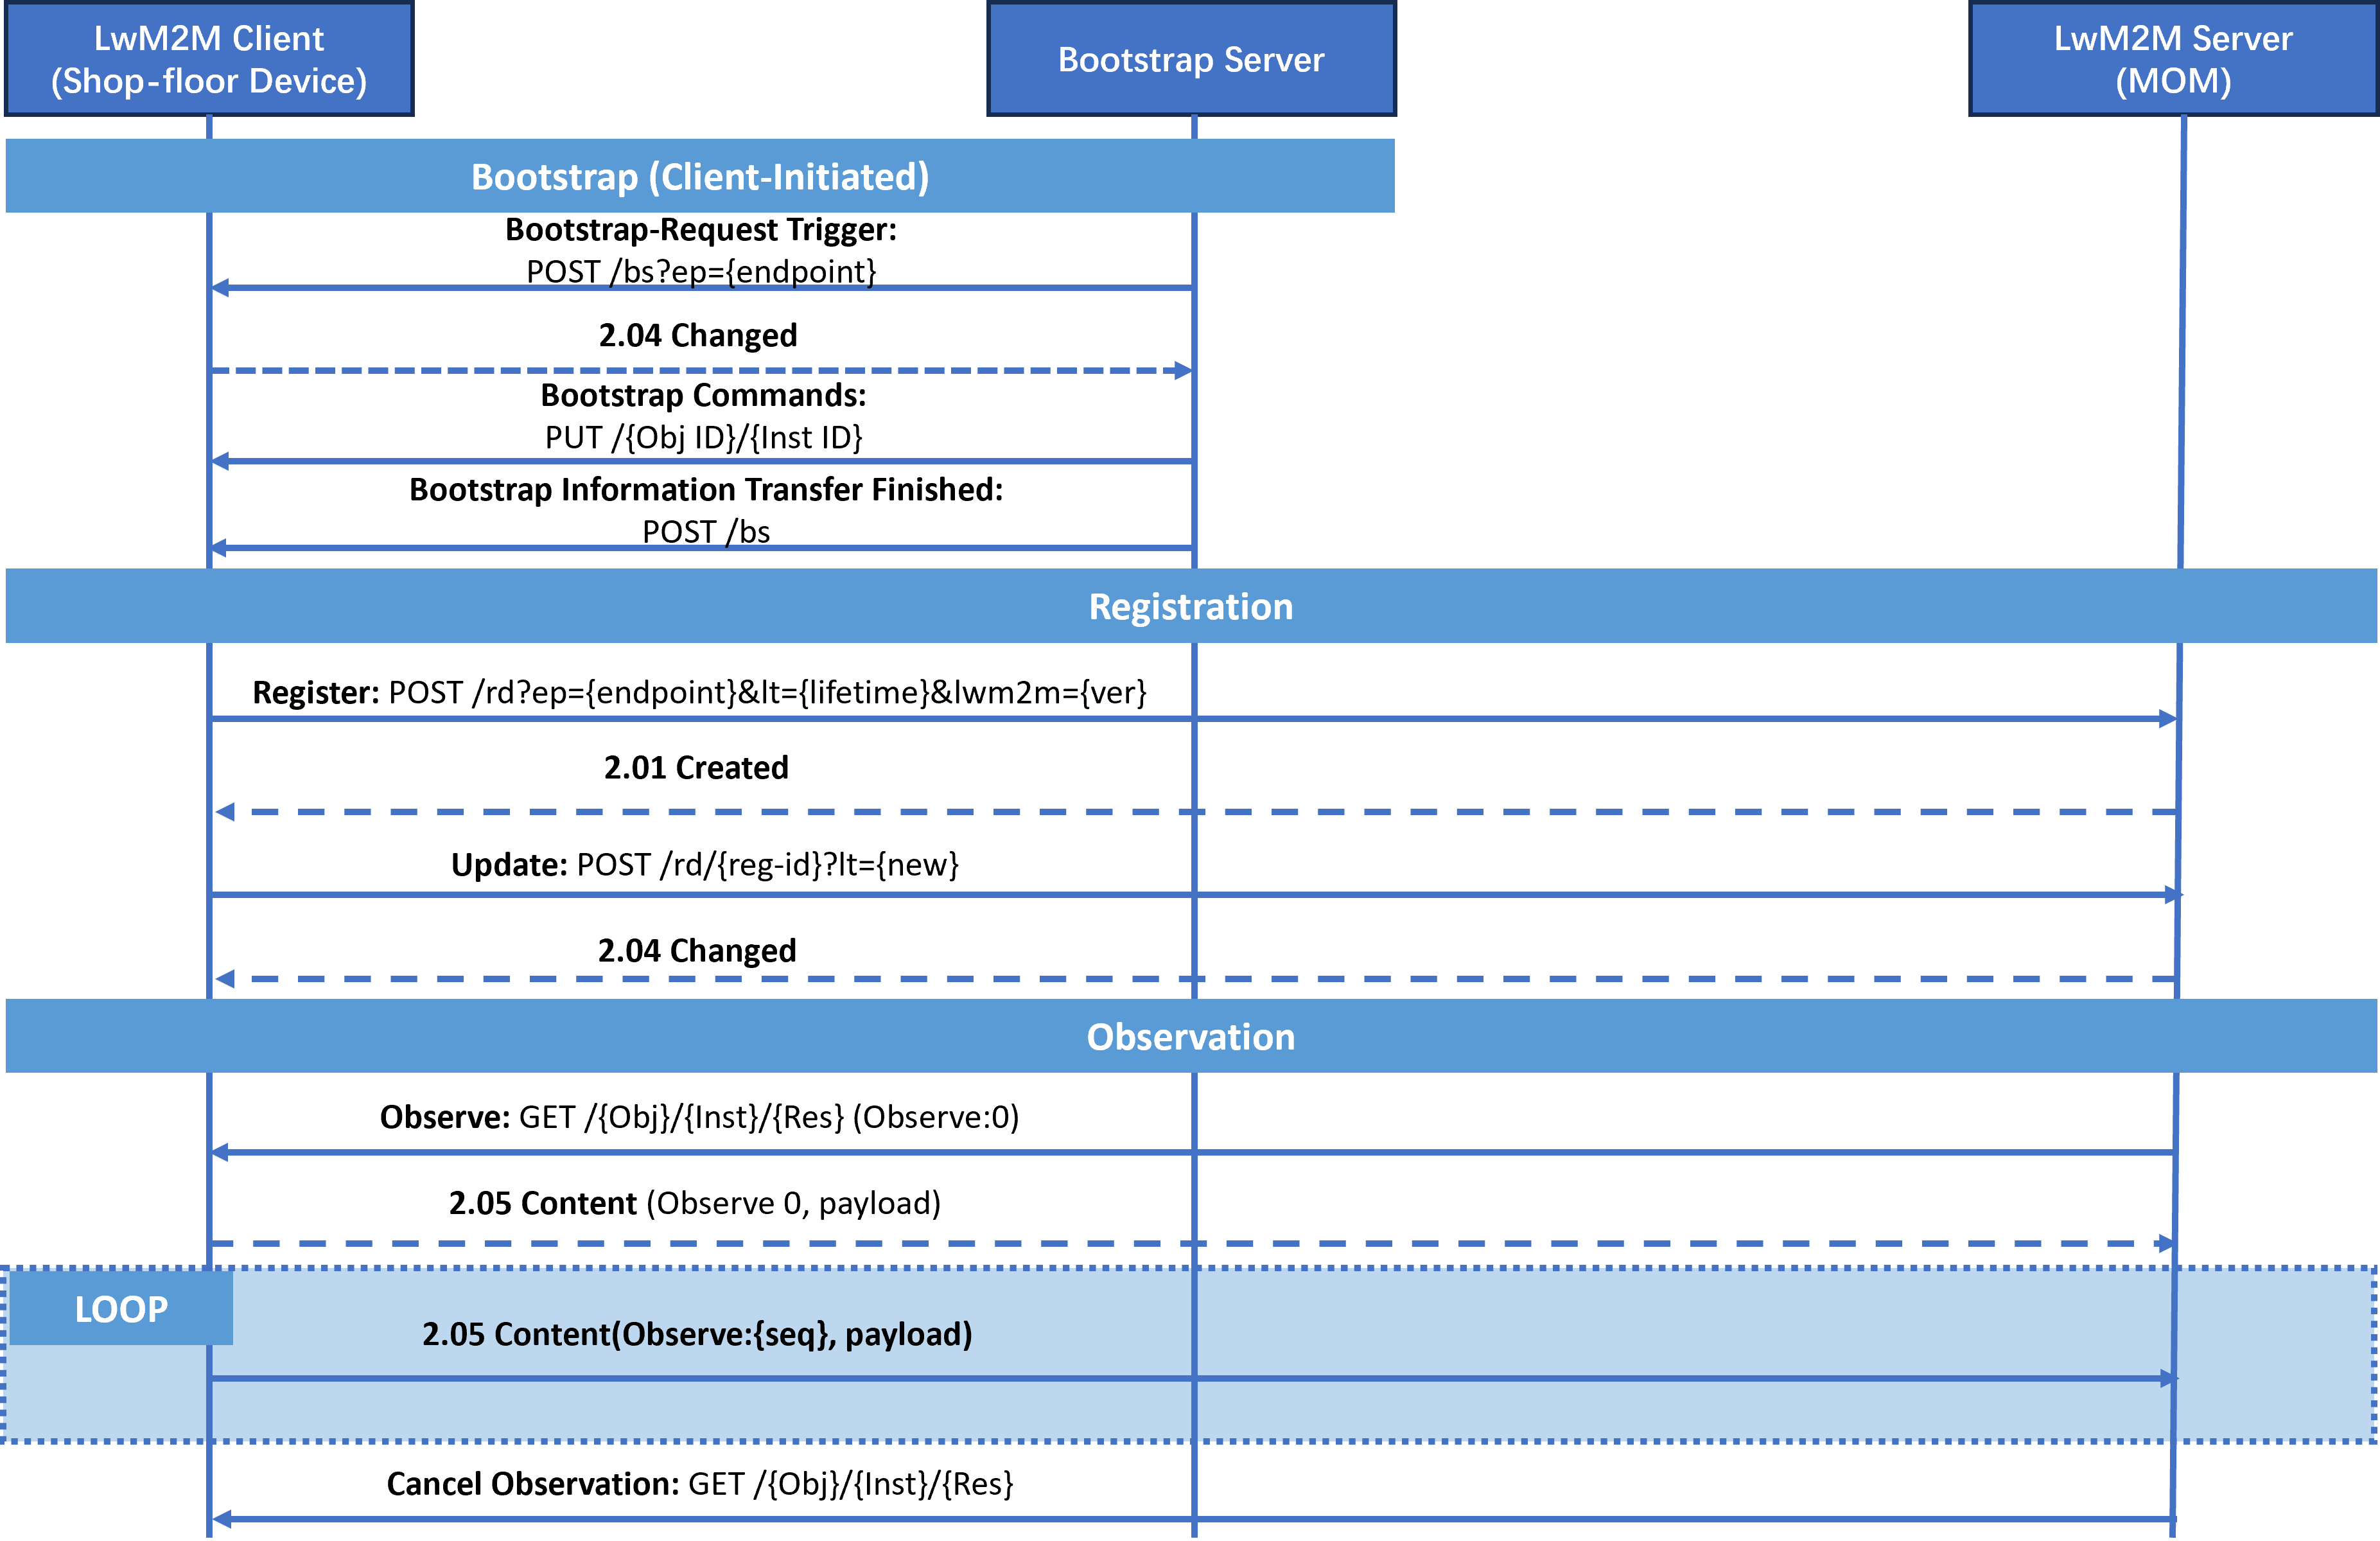
\includegraphics[width=0.75\textwidth]{figs/lwm2mseq.png}
	\caption{OMA LwM2M Communication Sequence.}
	\label{seq}
\end{figure}

The bootstrap phase begins with the Bootstrap Server sending a \path{POST /bs?ep={endpoint}} request. The client acknowledges, after which the server performs multiple PUT operations to write configuration objects (e.g., \path{Security Object /0/0}, \path{Server Object /1/0}). Finally, the server sends a \path{POST /bs (Bootstrap-Finish)} request.

After bootstrap, the client registers with the LwM2M Server by sending a \path{POST /rd?ep={endpoint}&lt={lifetime}&lwm2m={ver}} request, the server responds with \path{2.01 Created}. Optionally, the client may later send an update (\path{POST /rd/{reg-id}?lt={new}}); the server responds with \path{2.04 Changed}.

Observation is initiated by the server with a \path{GET /{Obj}/{Inst}/{Res} (Observe:0)} request. The client replies with a \path{2.05 Content} notification carrying the current resource value. When the resource changes (simulated by a periodic counter in the automaton), the client sends further asynchronous notifications. To stop the observation, the server sends a \path{GET /{Obj}/{Inst}/{Res} (Observe:1)} request.

In this work, we abstract the standard message exchange to retain only those interactions that affect the logical progression of the protocol. In particular, CoAP-level acknowledgments and retransmission mechanisms are omitted in this layer, as they do not influence functional correctness in a reliable communication setting. These aspects will be revisited in the probabilistic layer.

\subsection{Modeling of Core LwM2M Procedures}
To enable formal verification, the LwM2M protocol is modeled as a network of timed automata in UPPAAL. The system consists of two client automata and a set of server-side handlers, each responsible for one interface. All communications are modeled using synchronous channels, assuming reliable and loss-free message delivery.

\subsubsection{Abstract Data Structures}

\paragraph{Channels.}
Table~\ref{tab:channels} lists the channels used for synchronization between the client and the server automata. Each channel be mapped to one or multiple CoAP message(s) defined in the LwM2M specification. For example, \texttt{bootstrap\_start\_client[id]} models the Bootstrap‑Request. The channels are declared as arrays indexed by the client identifier, allowing the server to distinguish messages from different clients. The table also serves as a quick reference for readers to map the abstract channel names back to the original protocol messages.
\begin{table}[htbp]
\centering
\caption{Channels used in the functional model and their correspondence to LwM2M messages.}
\label{tab:channels}
\begin{tabular}{lll}
\toprule
\textbf{Channel} & \textbf{Direction} & \textbf{LwM2M Message} \\
\midrule
\texttt{bootstrap\_start\_client[id]}   & Server $\rightarrow$ Client & Bootstrap-Request Trigger \\
\texttt{bootstrap\_credential[id]}     & Client $\rightarrow$ Server & 2.04 Changed \\
\texttt{bootstrap\_config[id]}         & Server $\rightarrow$ Client & Bootstrap Commands \\
\texttt{bootstrap\_complete[id]}       & Client $\rightarrow$ Server & Bootstrap Information Transfer Finished \\
\midrule
\texttt{register\_start[id]}           & Client $\rightarrow$ Server & Register \\
\texttt{register\_objects[id]}         & Client $\rightarrow$ Server & Update \\
\texttt{register\_complete[id]}        & Server $\rightarrow$ Client & 2.01 Created \\
\midrule
\texttt{observe\_start[id]}            & Server $\rightarrow$ Client & Observe request \\
\texttt{notification[id]}              & Client $\rightarrow$ Server & Notification \\
\texttt{observe\_stop[id]}             & Server $\rightarrow$ Client & Cancel Observation \\
\bottomrule
\end{tabular}
\end{table}

\paragraph{Variables.}
The model uses a set of global and local variables to capture the state of each interface. The most important ones are listed in Table~\ref{tab:variables}. These variables track the progress of each client through the three interfaces and maintain the data needed for verification (e.g., resource values, counters). Together with the channels, they form the basis of the automata transitions.
\begin{table}[htbp]
\centering
\caption{Key global variables used in the functional model.}
\label{tab:variables}
\begin{tabular}{lp{0.65\linewidth}}
\toprule
\textbf{Variable} & \textbf{Description} \\
\midrule
\texttt{client\_state[id]} & Enumerated type representing the current phase of the client (e.g., \texttt{CLIENT\_STATE\_BOOTSTRAPPING}). \\
\texttt{client\_bootstrapped[id]} & Boolean indicating whether the client has successfully completed bootstrap. \\
\texttt{client\_registered[id]} & Boolean indicating whether the client has successfully registered. \\
\texttt{bootstrap\_completed\_count} & Counter incremented each time a client finishes bootstrap; used by the server to track progress. \\
\texttt{registration\_completed\_count} & Counter incremented each time a client finishes registration. \\
\texttt{observation\_cycle\_count} & Counter tracking the total number of notifications received; used in verification. \\
\texttt{resource\_value[id][res]} & Array modeling the value of a resource (e.g., temperature, production count). The client increments this value periodically to trigger notifications. \\
\texttt{observed\_resource[id]} & Index of the resource currently being observed by the client. \\
\bottomrule
\end{tabular}
\end{table}

\subsubsection{Client Automaton}
The client automaton (Fig.~\ref{cbase}) integrates the three interfaces in a single template. Its structure follows the communication flow and uses the state names listed in Table~\ref{tab:variables}.
\begin{figure}[pos=htbp]
	\centering
		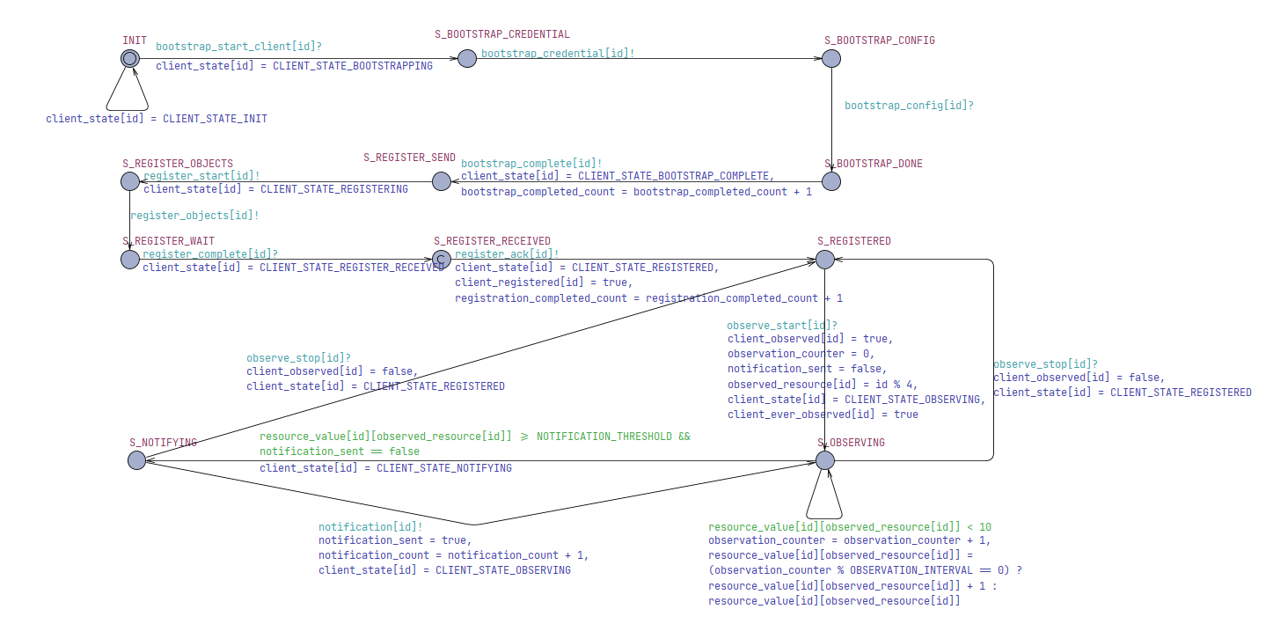
\includegraphics[width=0.98\textwidth]{figs/clientbaseline.png}
	\caption{Level 1 Client Model.}
	\label{cbase}
\end{figure}


\paragraph{Bootstrap.} The client starts in \texttt{INIT}. Upon receiving \texttt{bootstrap\_start\_client[id]?} from the server, it moves to \texttt{S\_BOOTSTRAP\_CREDENTIAL}. From there it sends its credentials \texttt{(bootstrap\_credential[id]!)} and enters \texttt{S\_BOOTSTRAP\_CONFIG}. After receiving \texttt{bootstrap\_config[id]?}, it sends \texttt{bootstrap\_complete[id]!} and finally reaches \texttt{S\_BOOTSTRAP\_DONE}. The entire exchange is instantaneous, because the functional model abstracts away time delays.

\paragraph{Registration.} Once bootstrap is finished, the client proceeds to \texttt{S\_REGISTER\_SEND}. It first sends two messages \texttt{register\_start[id]!} and \texttt{register\_objects[id]!} in sequence, then enters the state \texttt{S\_REGISTER\_WAIT}. Upon receiving \texttt{register\_complete[id]?}, it moves to the committed state \texttt{S\_REGISTER\_RECEIVED} and then to \texttt{S\_REGISTERED} after sending \texttt{register\_ack[id]!}. This sequence follows the OMA specification: the client first sends a registration request (possibly with an object list), the server acknowledges with a 2.01 Created response, and the client confirms with an ACK. Although the standard allows the Register‑Objects step to be combined with the initial registration, we keep them separate in the Level‑1 model, which preserves the ability to later refine the model without breaking the state machine.

\paragraph{Observation.} Once registered, the client may enter the observation phase upon receiving a subscription request from the server. The observation behavior is modeled as a cyclic interaction in which resource values evolve locally and may trigger notifications when a predefined threshold is reached. Instead of using explicit clocks, resource dynamics are simulated using a bounded counter. This provides a lightweight abstraction of time-dependent behavior while preserving the causal relationship between state changes and notifications.

To ensure finiteness of the model, observation is restricted to a bounded number of cycles. Each cycle consists of a notification followed by an explicit termination of the observation. Although real LwM2M observations may persist indefinitely, this bounded abstraction preserves the essential asynchronous reporting behavior while avoiding infinite state exploration. From \texttt{S\_REGISTERED}, the client may receive \texttt{observe\_start[id]?} and enter \texttt{S\_OBSERVING}. In this state, a resource value is simulated by a local counter \texttt{observation\_counter}. When the counter reaches the threshold \texttt{NOTIFICATION\_THRESHOLD} (set to 2), the client moves to \texttt{S\_NOTIFYING} and sends a \texttt{notification[id]!}. It then returns to \texttt{S\_OBSERVING}. The counter is incremented on a self‑loop edge, which is guarded by $resource\_value < 10$; this models the resource changing over time without introducing actual time (the guard is purely logical). The observation ends when the client receives \texttt{observe\_stop[id]?}, which brings it back to \texttt{S\_REGISTERED}.



\subsubsection{Server Automata}
Each server-side automaton is responsible for managing one interface and coordinates interactions with multiple clients.

\paragraph{Bootstrap Handler}  The bootstrap server, as shown in Fig.~\ref{bbase}, starts in \texttt{S\_IDLE} and immediately moves to the committed state \texttt{S\_SELECTING}. It then selects the next unprocessed client. For the selected client, it sends \texttt{bootstrap\_start\_client[current\_client]!}, then waits for \texttt{bootstrap\_credential[current\_client]?}, sends \texttt{bootstrap\_config[current\_client]!}, and finally waits for \texttt{bootstrap\_complete[current\_client]?}. After the completion, it increments the current client and repeats until all clients are processed, at which point it reaches \texttt{S\_ALL\_COMPLETE} and then \texttt{S\_FINAL\_IDLE}. 
\begin{figure}[pos=htbp]
	\centering
		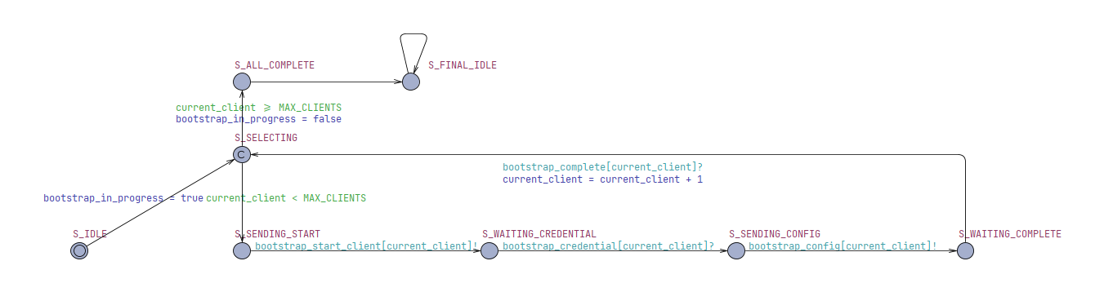
\includegraphics[width=0.98\textwidth]{figs/bootstraphandlerbaseline.png}
	\caption{Level 1 Bootstrap Handler Model.}
	\label{bbase}
\end{figure}


\paragraph{Registration Handler} The registration server follows a similar pattern but with the registration messages, as shown in Fig.~\ref{rbase}. It waits for bootstrap to finish (by checking \texttt{bootstrap\_completed\_count}), then enters a selection loop. For each client, it waits for \texttt{register\_start[current\_client]?} and \texttt{register\_objects[current\_client]?}, sends \texttt{register\_complete[current\_client]!}, and finally waits for \texttt{register\_ack[current\_client]?}. After all clients are registered, it goes to \texttt{S\_ALL\_REGISTERED} and then to \texttt{S\_FINAL\_IDLE}.

\begin{figure}[pos=htbp]
	\centering
		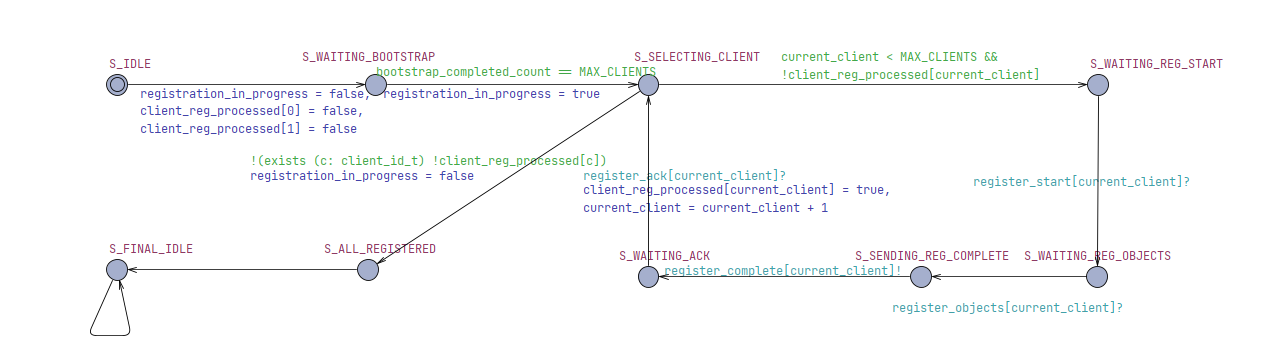
\includegraphics[width=0.9\textwidth]{figs/regsitrationhandlerbaseline.png}
	\caption{Level 1 Registration Handler Model.}
	\label{rbase}
\end{figure}

\paragraph{Observation Handler} The observation server cycles through a fixed number of times (\texttt{MAX\_OBSERVATION\_CYCLES}). For each client, it sends \texttt{observe\_start[selected\_client]!}, waits for a \texttt{notification[selected\_client]?}, and then sends \texttt{observe\_stop[selected\_client]!}. After completing all cycles, it reaches \texttt{S\_COMPLETED}. The counter $observation\_cycle\_count$ tracks the total number of received notifications and is used in verification.

\begin{figure}[pos=htbp]
	\centering
		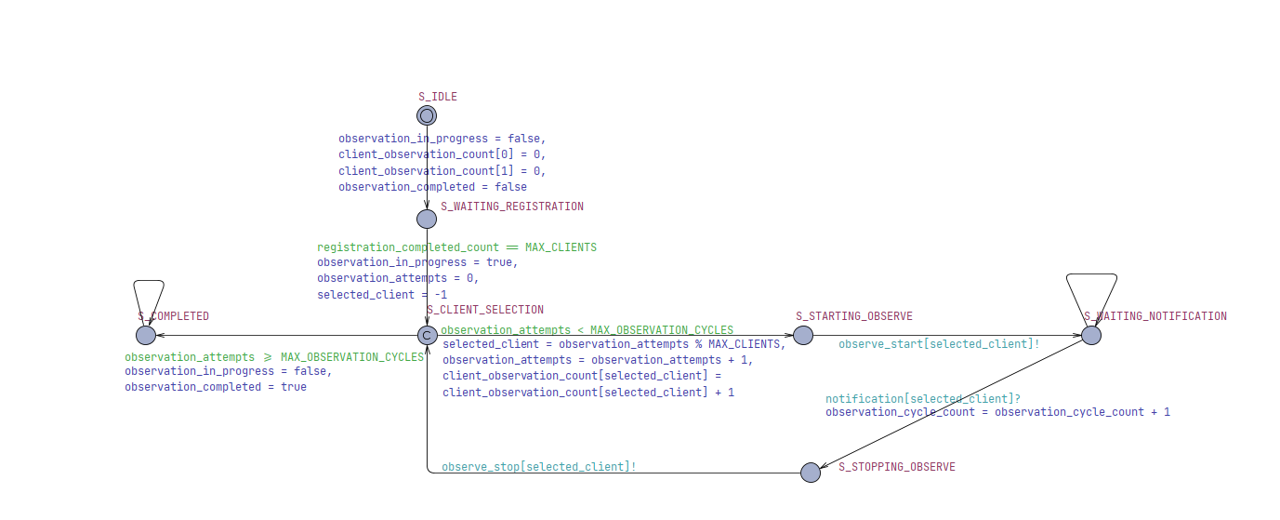
\includegraphics[width=0.98\textwidth]{figs/observationhandlerbaseline.png}
	\caption{Level 1 Observation Handler Model.}
	\label{obase}
\end{figure}

The three server automata are designed to execute in a fixed order (Bootstrap $\rightarrow$ Registration $\rightarrow$ Observation), following the natural life-cycle of a device in the industrial scenario. They do not employ clock constraints – the functional model assumes instantaneous communication – and rely entirely on synchronization through the channels defined in Table~\ref{tab:channels}.

The functional model deliberately abstracts several aspects of the real protocol to keep the state space small while preserving all behaviors that are relevant for functional correctness.

\begin{itemize}
    \item Message merging. The multiple PUT writes of the bootstrap phase are merged into a single \texttt{bootstrap\_config} message, because the exact sequence of writing individual objects does not affect the final state of the client (bootstrap completed). Similarly, the first notification of an observation is treated identically to subsequent notifications.
    \item Omitting CoAP acknowledgments. In a loss‑free environment, CoAP acknowledgments do not change the state of the automata; therefore they are omitted. They will be reintroduced in the probabilistic layer (Layer III) when we study message loss and retransmission.
    \item Urgent semantics. All states except the final ones (\texttt{S\_BOOTSTRAP\_DONE, S\_REGISTERED, S\_OBSERVING, S\_COMPLETED}) are declared urgent (invariant $x \leq 0$). This forces time to freeze during message exchanges, which is acceptable because the functional model is only concerned with the logical sequence of events, not with timing.
\end{itemize}

These abstractions are justified by the fact that they do not influence the core functional properties we intend to verify: reachability of final states, mutual exclusion, and deadlock freedom. The resulting automata are therefore faithful to the protocol’s intended behavior while remaining small enough for exhaustive verification.

\subsection{Functional Property Verification}
We verify the functional correctness of the LwM2M model using the standard UPPAAL model checker. The properties are expressed in TCTL and are taken directly from the queries in the Level‑1 implementation. Table~\ref{tab:func-props} summarizes the verified properties and their outcomes. All properties are satisfied, confirming that the model correctly implements the intended protocol behavior.

The verified properties cover three categories:
\begin{itemize}
\item \textbf{Reachability} (e.g., Bootstrap completion) ensures that each interface can eventually reach its intended final state.
\item \textbf{Safety} (e.g., deadlock freedom) guarantees that the system never enters an undesirable state where no further progress is possible or where concurrent operations interfere incorrectly.
\item \textbf{Boundedness} (e.g., notification count bound) ensures that the finite abstraction of the observation cycles does not cut off legitimate behavior.
\end{itemize}
The successful verification of these properties provides a solid baseline for the subsequent security and performance layers.

\begin{table}[!htb]
\centering
\caption{Verification results of functional properties.}
\label{tab:func-props}
\small
\begin{tabularx}{\linewidth}{lLc}
\toprule
\textbf{Property} & \textbf{TCTL Formula} & \textbf{Result} \\
\midrule
Bootstrap completion (both clients) &
\texttt{E<> (Client1.S\_BOOTSTRAP\_DONE \&\& Client2.S\_BOOTSTRAP\_DONE)} & \checkmark \\
Registration completion (both clients) &
\texttt{E<> (Client1.S\_REGISTERED \&\& Client2.S\_REGISTERED)} & \checkmark \\
Observation completion &
\texttt{E<> (ObservationHandler1.S\_COMPLETED)} & \checkmark \\
Deadlock freedom &
\texttt{A[] not deadlock} & \checkmark \\
Notification count bound &
\texttt{A[] (notification\_count <= MAX\_OBSERVATION\_CYCLES)} & \checkmark \\
\bottomrule
\end{tabularx}
\end{table}

\paragraph{Remark (Trace inclusion via interface projection).}
The functional model (Layer I) integrates Bootstrap, Registration, and Observation into a single automaton, while the security and performance models (Layers II and III) treat each interface separately. To compare their behaviors, we consider the projection of a full system trace onto the messages belonging to a particular interface. Let $\mathcal{T}_{\text{func}}^{(I)}$ denote the set of all such projected traces for interface $I$ (where $I \in {\text{Bootstrap}, \text{Registration}, \text{Observation}}$) in the functional model.
For each interface, the corresponding security model (Layer II) is built by adding attacker automata to the functional interface model, without deleting or modifying the original transitions. Therefore, every projected trace of the functional interface is also a trace of the security interface model:
$$\mathcal{T}_{\text{func}}^{(I)} \subseteq \mathcal{T}_{\text{sec}}^{(I)}$$

Similarly, the performance model (Layer III) extends the functional interface model with probabilistic branches and delays, preserving all original deterministic traces as positive‑probability traces:
$$\mathcal{T}_{\text{func}}^{(I)} \subseteq \mathcal{T}_{\text{perf}}^{+,(I)}$$

These per‑interface inclusions ensure that functional properties proved on an isolated interface (e.g., deadlock freedom, reachability of final states) remain valid when the interface is embedded in the full system and when it is extended with attackers or probabilistic behavior. The overall correctness of the integrated system follows from the fact that the three interfaces are executed sequentially and do not interfere with each other’s channels.

\section{Security Layer: Security-Enhanced Model with Attackers}
To evaluate the resilience of LwM2M against realistic threats, we extend the functional models with dedicated attacker automata that run in parallel with the original components. Each attacker is designed to observe and interfere with the communication channels that carry the critical messages of the corresponding interface. The attacks are modeled as separate timed automata that can be activated or deactivated by a global mode variable, allowing us to compare the behavior of the system with and without the attacker.

We consider three interfaces: Bootstrap, Registration, and Observation. For each interface we identify the most relevant threats based on the LwM2M security analysis~\cite{Sasi2024} and on common IoT attack patterns. Table~\ref{tab:attacks} summarizes the attacks modeled for each interface. 
\begin{table}[htbp]
\centering
\caption{Security attacks modeled for each LwM2M interface.}
\label{tab:attacks}
\begin{tabular}{llp{0.55\linewidth}}
\toprule
\textbf{Interface} & \textbf{Attack Type} & \textbf{Description} \\
\midrule
Bootstrap   & MITM (Man-in-the-Middle)   & Attacker intercepts the configuration message, replaces it with a tampered value, and forwards it to the client.  \\
            & Fake Bootstrap Server      & Attacker impersonates the bootstrap server and sends malicious configuration requests. \\
\midrule
Registration & Replay                    & Attacker records a valid registration request and later replays it to the server, causing duplicate registrations. \\
             & Denial of Service (DoS)   & Attacker floods the server with registration requests, exhausting resources and triggering throttling. \\
\midrule
Observation  & Notification Tampering    & Attacker intercepts a notification, modifies its payload, and forwards the altered message to the server. \\
             & Notification Replay       & Attacker records a notification and replays it later, causing the server to receive stale data. \\
\bottomrule
\end{tabular}
\end{table}

Because the observation interface involves periodic notifications and thus offers a richer attack surface, we describe its security model in detail. The attacks on Bootstrap and Registration are summarized more concisely, as they follow similar patterns. For brevity, we do not present the full UPPAAL automata for every attacker variant in the paper. Instead, we illustrate the most representative attacker (the tampering attacker for Observation) and briefly describe the others. The complete set of UPPAAL models, including all automata, global declarations, and verification queries, is available in the supplementary material at: \url{https://github.com/celine-celine/Hierarchical-Verification-of-LwM2M-Using-UPPAAL-UPPAAL-SMC}.

\subsection{Observation Security Model}
The observation interface is used for asynchronous reporting of resource values. A typical scenario involves the server subscribing to a resource (e.g., temperature) and the client sending notifications whenever the value changes. An attacker can attempt to (1) \textbf{tamper} with the notification payload, or (2) \textbf{replay} old notifications, or (3) \textbf{inject} fake notifications. We focus on tampering and replay, as they are the most relevant for data integrity.

\subsubsection{Threat Modeling} 
We extend the functional observation model with two attacker automata:
\begin{itemize}
    \item \textbf{Tampering attacker} intercepts a notification message, modifies its payload (e.g., changes the reported value), and forwards the altered message to the server.
    \item \textbf{Replay attacker} records a legitimate notification and later re-sends it, causing the server to receive stale data.
\end{itemize}

Both attackers run in parallel with the client and the observation handler. They are activated by setting a global variable \texttt{attack\_mode} to \texttt{TAMPER\_NOTIFY} or \texttt{REPLAY\_NOTIFY}. When inactive, the system behaves exactly as in the functional model.

\subsubsection{Tampering Attacker}
The tampering attacker is modeled as a timed automaton (Fig.~\ref{tamper}) with the following states:
\begin{figure}[pos=htbp]
	\centering
		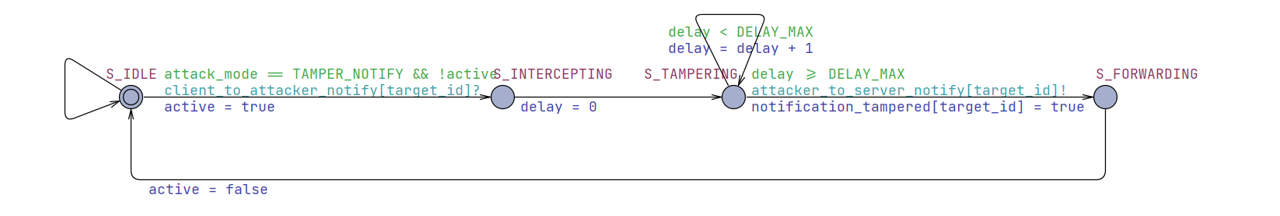
\includegraphics[width=0.9\textwidth]{figs/observationtamper.png}
	\caption{Observation Tamper Attacker.}
	\label{tamper}
\end{figure}

\begin{itemize}
    \item \texttt{S\_IDLE}: initial state, waiting for a notification message from the client.
    \item \texttt{S\_INTERCEPTING}: after receiving the original notification, the attacker stores the message.
    \item \texttt{S\_TAMPERING}: the attacker introduces a small delay (simulating processing) and then replaces the payload with a tampered value.
    \item \texttt{S\_FORWARDING}: the attacker sends the tampered notification back to the server using the original channel \texttt{notification[selected\_client]!}.
\end{itemize}

The attacker uses additional channels \texttt{client\_to\_attacker\_notify} to receive the original notification from the client and \texttt{attacker\_to\_server\_notify} to forward the tampered version. The observation handler is extended to accept notifications from either the original channel or the attacker’s channel, depending on the attack mode. A global flag \texttt{notification\_tampered[id]} records whether a notification has been tampered for a given client.
\paragraph{Verification.} We verify the following properties using the standard UPPAAL model checker. \textbf{Attack reachability}:  $E\langle\rangle\; (\texttt{attack\_mode == TAMPER\_NOTIFY} \land \texttt{notification\_tampered[0]})$. This property checks whether a tampered notification can ever be observed. The verification succeeds, confirming that the tampering attacker can successfully inject a falsified notification.

\subsubsection{Replay Attacker} 
The replay attacker is simpler: it records a notification message when it first appears, then after a random delay (simulated by a bounded counter) it re-sends the exact same message via a dedicated channel \texttt{attacker\_to\_server\_replay}. The observation handler accepts these replayed messages when the attack mode is \texttt{REPLAY\_NOTIFY}. A counter \texttt{replay\_count} is incremented each time a replay is sent.

\paragraph{Verification.} We check the following property to show that the replay attacker can indeed replay a notification:
$E\langle\rangle\; (\texttt{attack\_mode == REPLAY\_NOTIFY} \land \texttt{replay\_count} > 0)$ holds, indicating that replays are feasible.

Moreover, because the original model does not include any sequence‑number or freshness check, the server cannot distinguish the replayed notification from a fresh one. This vulnerability will be addressed in the performance layer by introducing OSCORE, which provides sequence numbers and message authentication.

\subsection{Trace Inclusion for the MITM Attacker}
\label{sec:remark-mitm}

Let $\Sigma$ be the set of all channel synchronization actions (e.g., $\texttt{notification!}$, $\texttt{observe\_start?}$). 
A \emph{trace} $\sigma = a_1 a_2 \dots a_n$ is a finite sequence of actions. 
Denote by $\mathcal{T}(M)$ the set of all finite traces of a model $M$.

The functional observation model $M_{\text{func}}$ uses the original channel set, namely:

$C_{\text{orig}} = \{\texttt{notification}, \texttt{observe\_start}, \texttt{observe\_stop}\}$. 

The security model $M_{\text{sec}}$ extends $M_{\text{func}}$ with the MITM attacker automaton $A_{\text{mitm}}$ and introduces new channels 
$C_{\text{new}} = \{\texttt{client\_to\_attacker\_notify}, \texttt{attacker\_to\_server\_notify}\}$. 
All transitions on $C_{\text{orig}}$ are identical in $M_{\text{func}}$ and $M_{\text{sec}}$; $A_{\text{mitm}}$ only synchronizes on $C_{\text{new}}$ and starts in its idle location.


$$\mathcal{T}(M_{\text{func}}) \subseteq \mathcal{T}(M_{\text{sec}})$$
\begin{proof}[Proof sketch]
Take any $\sigma \in \mathcal{T}(M_{\text{func}})$. In $M_{\text{sec}}$, keep $A_{\text{mitm}}$ in its idle location throughout the execution. 
Execute the transitions of $\sigma$ exactly as in $M_{\text{func}}$; they only involve channels in $C_{\text{orig}}$, which are untouched by $A_{\text{mitm}}$. 
Hence $\sigma$ is also a trace of $M_{\text{sec}}$. 
\end{proof}

The same reasoning applies to all other attackers (eavesdropper, fake BS, replay, DoS, etc.) because they are all constructed by adding new channels without modifying existing transitions.


\subsection{Bootstrap Security Model}
The bootstrap procedure initializes a device with security credentials and server information. We model two attacks:
\begin{itemize}
    \item \textbf{MITM (Man‑in‑the‑Middle)}: an attacker intercepts the configuration message, replaces it with a tampered value, and forwards it to the client.
    \item \textbf{Fake Bootstrap Server}: an attacker impersonates the bootstrap server and sends malicious configuration requests.
\end{itemize}

Each attack is modeled as a separate automaton intercepting the corresponding channels (e.g., \texttt{bootstrap\_config}). The verification confirms that both attacks are feasible and that the client cannot complete bootstrap successfully when attacked. Detailed results are summarized in Table~\ref{tab:sec-verification}.

\subsection{Registration Security Model}
The registration interface is susceptible to replay attacks and Denial‑of‑Service (DoS) attacks. The replay attacker records a valid \texttt{register\_start} message and later replays it; the server, lacking sequence‑number verification, accepts the duplicate. The DoS attacker floods the server with registration requests, exhausting resources and triggering a throttling mechanism. Verification shows that both attacks can be carried out.


\subsection{Verification Result and Analysis}
Table~\ref{tab:sec-verification} summarizes the verification results for all three interfaces. All properties are satisfied, confirming that the modeled attacks can indeed be successfully carried out, exposing vulnerabilities in terms of integrity, authentication, and freshness.

\begin{table}[htbp]
\centering
\caption{Verification results of security properties for each LwM2M interface.}
\label{tab:sec-verification}
\begin{tabularx}{\linewidth}{lXc}
\toprule
\textbf{Interface} & \textbf{Verified Property} & \textbf{Result} \\
\midrule
\multirow{6}{*}{Bootstrap}
 & \textbf{Attack reachability:} $E\langle\rangle\; (\texttt{attack\_mode == MITM\_ATTACK} \land \texttt{message\_tampered[0]})$ & \checkmark \\
 & \textbf{Security invariant:} $A[]\; (\texttt{attack\_mode == MITM\_ATTACK} \land \texttt{message\_tampered[0]} \Rightarrow \lnot\texttt{client\_bootstrapped[0]})$ & \checkmark \\
 & \textbf{Fake BS reachability:} $E\langle\rangle\; (\texttt{attack\_mode == FAKE\_BS\_ATTACK} \land \texttt{client\_bs\_type[0]} = 2 \land \texttt{client\_state[0]} = \texttt{CLIENT\_STATE\_ERROR})$ & \checkmark \\
 & \textbf{Fake BS safety:} $A[]\; (\texttt{attack\_mode == FAKE\_BS\_ATTACK} \land \texttt{client\_bs\_type[0]} = 2 \Rightarrow \lnot\texttt{client\_bootstrapped[0]})$ & \checkmark \\
 & \textbf{Authenticity:} $A[]\; (\texttt{attack\_mode == FAKE\_BS\_ATTACK} \land \texttt{client\_bootstrapped[0]} \Rightarrow \texttt{client\_bs\_type[0]} = 1)$ & \checkmark \\
\midrule
\multirow{4}{*}{Registration}
 & \textbf{Replay reachability:} $E\langle\rangle\; (\texttt{attack\_mode == REPLAY\_ATTACK} \land \texttt{attack\_detected})$ & \checkmark \\
 & \textbf{Replay liveness:} $E\langle\rangle\; (\texttt{attack\_mode == REPLAY\_ATTACK} \land \exists c: \texttt{client\_registered[c]})$ & \checkmark \\
 & \textbf{DoS reachability:} $E\langle\rangle\; (\texttt{attack\_mode == DOS\_ATTACK} \land \texttt{dos\_throttling\_active})$ & \checkmark \\
 & \textbf{DoS liveness}: $E\langle\rangle\; (\texttt{attack\_mode == DOS\_ATTACK} \land \lnot\texttt{dos\_throttling\_active} \land \exists c: \texttt{client\_registered[c]})$ & \checkmark \\
\midrule
\multirow{3}{*}{Observation}
 & \textbf{Tampering reachability:} $E\langle\rangle\; (\texttt{attack\_mode == TAMPER\_NOTIFY} \land (\texttt{notification\_tampered[0]} \lor \texttt{notification\_tampered[1]}))$ & \checkmark \\
 & \textbf{Observation liveness:} $E\langle\rangle\; (\texttt{attack\_mode == TAMPER\_NOTIFY} \land \texttt{ObservationHandler1.S\_COMPLETED})$ & \checkmark \\
 & \textbf{Replay reachability:} $E\langle\rangle\; (\texttt{attack\_mode == REPLAY\_NOTIFY} \land \texttt{replay\_count} > 0)$ & \checkmark \\
\bottomrule
\end{tabularx}
\end{table}

\textbf{Bootstrap.} The MITM attacker can tamper with the configuration message, and the invariant shows that a tampered client never becomes bootstrapped. The fake BS attacker successfully leads the client into an error state, while the authenticity property ensures that any successfully bootstrapped client must have communicated with the legitimate server. These results expose the lack of message integrity and server authentication in the bootstrap procedure.

\textbf{Registration.} The replay attacker can cause duplicate registrations, and the DoS attacker can trigger throttling. However, the liveness property shows that even under DoS, some clients can still register, indicating that the throttling mechanism is not completely destructive. Nevertheless, the absence of sequence numbers makes replay attacks possible.

\textbf{Observation.} Both notification tampering and replay are reachable. The server may receive falsified resource values (tampering) or stale data (replay), undermining the reliability of the observation interface.

These vulnerabilities motivate the introduction of security mechanisms—DTLS for bootstrap/registration and OSCORE for observation—which will be evaluated in the next layer under probabilistic network conditions.

\section{Performance Layer: Stochastic Performance Model}
While the functional and security layers assume reliable communication, real‑world networks are inherently unreliable. Packets may be lost, delayed, or reordered, and these effects can significantly impact the performance of IoT protocols. In this layer we therefore extend our LwM2M models with probabilistic behavior, enabling us to evaluate the system’s performance under realistic network conditions. We use UPPAAL SMC (Statistical Model Checking), which supports randomized choices and statistical inference, to estimate quantities such as the probability of successful completion, the number of retransmissions, and the impact of security mechanisms.

Because the observation interface involves periodic notifications and thus offers a rich set of performance metrics, we describe its probabilistic model in detail. The models for Bootstrap and Registration are then summarized more concisely, as they follow the same methodological pattern.

\subsection{Observation Probabilistic Model}
\subsubsection{Model Extension}
We start from the functional observation model and add three probabilistic elements:
\begin{itemize}
    \item \textbf{Packet loss}: messages may be dropped independently with a fixed probability $p_{loss}$. Based on empirical studies of LwM2M in industrial environments~\cite{ge2019design}, we set $p_{loss} = 0.005$ ($0.5\%$).
    \item \textbf{Message retransmission}: the client can send notifications as CON (confirmable) messages. If an acknowledgment (ACK) is not received within a timeout, the client retransmits the message up to a maximum number of times. We follow the CoAP standard: initial $timeout = 50 ms$, exponential back‑off, maximum $4$ retransmissions~\cite{shelby2014rfc}.
    \item \textbf{Security overhead}: when the optional security mechanism (OSCORE) is enabled, we add a fixed processing delay for encryption and decryption ($5 ms$ and $4 ms$ respectively).
    This estimation is based on experimental studies: Gunnarsson et al. demonstrate that OSCORE displays moderately better performance than TinyDTLS with no additional performance penalty ~\cite{gunnarsson2021evaluating}. Complementary low-level evaluations of OSCORE libraries on constrained microcontrollers report per‑message processing times in the low millisecond range ~\cite{gundougan2020iot}. Our chosen values are well within this range and are further scaled to match the time granularity of our UPPAAL model.
\end{itemize}

All timing parameters are expressed in milliseconds; the model uses real‑valued clocks to capture the passage of time. The loss and retransmission behavior is implemented by replacing the original deterministic notification channel with a probabilistic branch inside the client automaton.

\subsubsection{Client Automaton (Probabilistic)}
The client automaton (Fig.~\ref{smcobservation}) is extended with a branch point that decides whether a notification is successfully sent or lost. The sending path also includes an optional encryption delay when OSCORE is enabled.

\begin{figure}[pos=htbp]
	\centering
		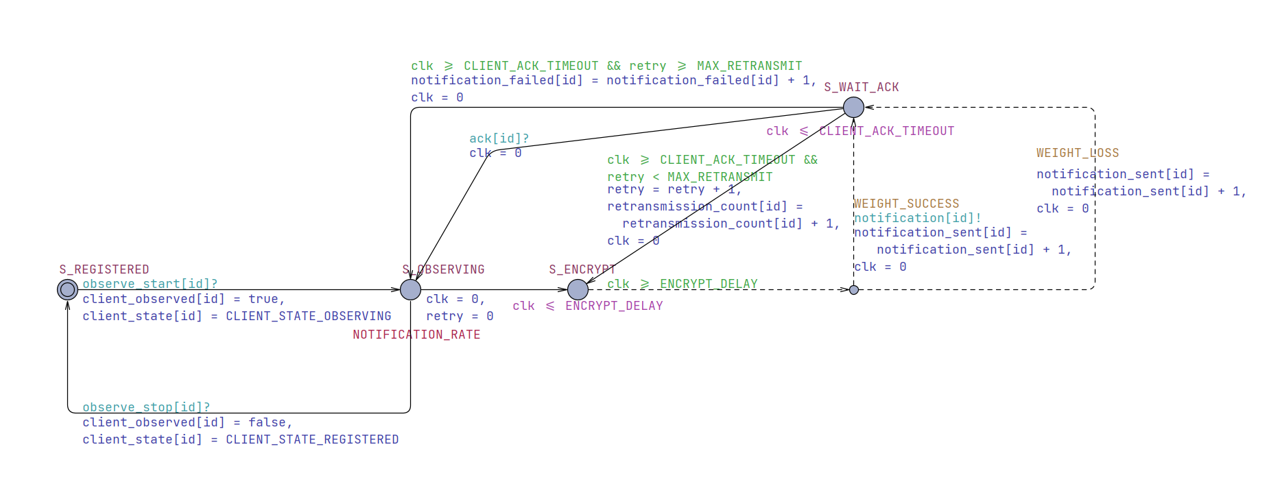
\includegraphics[width=0.9\textwidth]{figs/clientsmcretrans.png}
	\caption{Observation Client Model with Packet Loss and Retransmission Mechanism.}
	\label{smcobservation}
\end{figure}

\begin{itemize}
    \item From \texttt{S\_OBSERVING} to \texttt{S\_ENCRYPT}: triggered by the rate \texttt{NOTIFICATION\_RATE} ($0.01 ms^{-1}$, i.e., average interval $100ms$). The client moves to an encryption state where it spends \texttt{ENCRYPT\_DELAY} time units if OSCORE is enabled; otherwise it proceeds directly to the send branch.
    \item Send branch: the client either actually sends the notification (probability $1-p_{loss}$) or drops it (probability $p_{loss}$). In the sending case, it broadcasts the message and then enters a waiting state to receive the ACK.
    \item Wait for ACK: if a CON message was sent, the client waits for the server’s ACK. If the ACK arrives within the timeout, the notification is considered successful. If not, the client retransmits (up to $MAX\_RETRANSMIT = 4 $), each time doubling the timeout.
\end{itemize}

\subsubsection{Observation Handler (Probabilistic)}
The server automaton is modified to handle CON notifications and to record the reception of notifications. It now has a waiting state with an invariant that allows time to pass, enabling the timeout mechanism. The server also includes a decryption delay when OSCORE is enabled. The reception of a notification increments a counter \texttt{notification\_received}; the server sends an ACK (which is assumed to be reliably delivered, to limit state-space growth). A timeout edge moves the server back to the client selection state if no notification arrives within the allowed time window.

\subsubsection{Parameters and Experimental Setup}
All experiments use the parameters listed in Table~\ref{tab:perf-params}. The simulation time bound is set to $21000 ms$, which is long enough to observe several hundred notification events. We run $200$ independent simulations for each configuration; the results are reported with $95\%$ confidence intervals.
\begin{table}[htbp]
\centering
\caption{Parameters used in the probabilistic models.}
\label{tab:perf-params}
\begin{tabular}{llp{0.6\linewidth}}
\toprule
\textbf{Parameter} & \textbf{Value} & \textbf{Description} \\
\midrule
\texttt{NOTIFICATION\_RATE} & 0.01ms$^{-1}$ & Mean notification interval (100ms) \\
\texttt{LOSS\_PROB} & 0.005 & Packet loss probability (0.5\%) \\
\texttt{MAX\_RETRANSMIT} & 4 & Maximum number of retransmissions \\
\texttt{ACK\_TIMEOUT} & 50ms & Initial ACK timeout for CON messages \\
\texttt{ENCRYPT\_DELAY} & 5ms & OSCORE encryption delay \\
\texttt{DECRYPT\_DELAY} & 4ms & OSCORE decryption delay \\
\texttt{DTLS\_HANDSHAKE\_DELAY} & 80ms & DTLS handshake delay (once per client) \\
\texttt{DTLS\_ENCRYPT\_DELAY} & 6ms & DTLS message encryption delay \\
\texttt{DTLS\_DECRYPT\_DELAY} & 5ms & DTLS message decryption delay \\
\texttt{SIM\_TIME} & 21000ms & Simulation time bound \\
\texttt{SIM\_RUNS} & 200 & Number of independent simulations \\
\bottomrule
\end{tabular}
\end{table}

\subsubsection{Verified Properties}
We consider three experimental configurations:
\begin{itemize}
    \item \textbf{A (no security, no retransmission)}: baseline where notifications are sent as NON messages without loss recovery.
    \item \textbf{B (OSCORE only, no retransmission)}: same as A but with encryption/decryption delays added.
    \item \textbf{C (OSCORE + retransmission)}: notifications are sent as CON messages with full retransmission logic.
\end{itemize}

For each configuration we estimate the following quantities using UPPAAL SMC:
\begin{itemize}
    \item \textbf{Success probability}: the probability that the server receives at least one notification within the time bound.
    \item \textbf{Throughput}: the expected number of notifications successfully delivered.
    \item \textbf{Retransmission count}: the expected number of retransmissions (only for configuration C)
\end{itemize}

The queries are expressed in the SMC language as:
\[
\begin{aligned}
&\texttt{Pr[<=21000;200] (<> notification\_received[0] > 0)}\\
&\texttt{E[<=21000;200] (max: notification\_received[0])}\\
&\texttt{E[<=21000;200] (max: retransmission\_count)}
\end{aligned}
\]

\subsubsection{Verification Results}
Table ~\ref{tab:obs-perf-results} summarizes the results for the three configurations. The values are given as the estimate ± the half‑width of the $95\%$ confidence interval.
\begin{table}[htbp]
\centering
\caption{Performance evaluation results for the observation interfaces. Values are given as estimate $\pm$ half‑width of the $95\%$ confidence interval.}
\label{tab:obs-perf-results}
\begin{tabular}{llccc}
\toprule
\textbf{Interface} & \textbf{Configuration} & \textbf{Success Probability} & \textbf{Throughput (max notifications)} & \textbf{Retransmissions (max)} \\
\midrule
\multirow{3}{*}{Observation}
 & A & 0.9926 ± 0.0070 & 1033.5 ± 2.74 & – \\
 & B & 0.9926 ± 0.0070 & 958.2 ± 2.63  & – \\
 & C & 1.0000 ± 0.0000 & 984.5 ± 2.84  & 0.005 ± 0.010 \\
\bottomrule
\end{tabular}
\end{table}

From data collect above, we come to the following conclusions. First of all, the success probability remains high in all configurations, because even without retransmission the packet loss probability is low ($0.5\%$). Moreover, OSCORE introduces a noticeable overhead: the throughput drops from $1033$ to $958$ notifications, i.e., a reduction of about $7\%$. This overhead is due to the fixed encryption/decryption delays. Finally, with retransmission (configuration C), the success probability becomes $1$ (within the confidence interval), and the throughput partially recovers to $984$. The very small retransmission count ($0.005$) shows that retransmissions are rarely needed but are effective when they occur.

These results demonstrate that while OSCORE adds a modest performance penalty, combining it with retransmission can completely compensate for the packet loss, achieving near‑perfect reliability.


\paragraph{Remark (Trace preservation in the probabilistic model).}
The performance model $M_{\text{perf}}$ extends the functional model $M_{\text{func}}$ with:
\begin{itemize}
    \item probabilistic packet loss (a branch with weight $5$ vs. $995$ for successful sending),
    \item CoAP‑style retransmissions (timeout and retry logic),
    \item security overhead delays (DTLS/OSCORE encryption and decryption).
\end{itemize}
However, the functional behavior is recovered as the special case where:
\begin{itemize}
    \item no packet loss occurs (the successful‑send branch is taken),
    \item no retransmissions are triggered (the first transmission succeeds immediately),
    \item security mechanisms are disabled (encryption/decryption delays are zero).
\end{itemize}
For any trace $\sigma \in \mathcal{T}(M_{\text{func}})$, we can execute the same sequence of transitions in $M_{\text{perf}}$ by always choosing the successful‑send branch, avoiding any timeout (the ACK arrives within the timeout), and setting the security delays to zero. Since the successful‑send branch has weight $995 > 0$, the absence of retransmissions is a particular deterministic behavior, and security can be disabled by a global flag, the trace $\sigma$ occurs with positive probability in $M_{\text{perf}}$. Therefore,
\[
\mathcal{T}(M_{\text{func}}) \subseteq \mathcal{T}^+(M_{\text{perf}}).
\]

\subsection{Bootstrap and Registration Probabilistic Models}
The probabilistic models for Bootstrap and Registration follow the same design pattern as Observation, but they are much simpler because these interfaces do not involve periodical operations. 

In the Bootstrap model, both the client and the server implement a full CoAP retransmission mechanism (Fig.~\ref{smcbootstrap}). The client sends the initial \texttt{bootstrap\_start} as a CON message and enters a waiting state. If no ACK is received within the initial timeout (50ms), it retransmits the request up to four times, doubling the timeout each time. The server, after receiving the request, sends an ACK and then proceeds to send the configuration as a CON message. It also waits for an ACK from the client and retransmits the configuration if necessary. This bidirectional reliability logic is captured by adding waiting states (\texttt{S\_WAIT\_ACK}) and timeout edges in both automata. The handshake and encryption delays of DTLS are inserted before the first request and after the reception of the configuration, respectively.

\begin{figure}[pos=htbp]
	\centering
		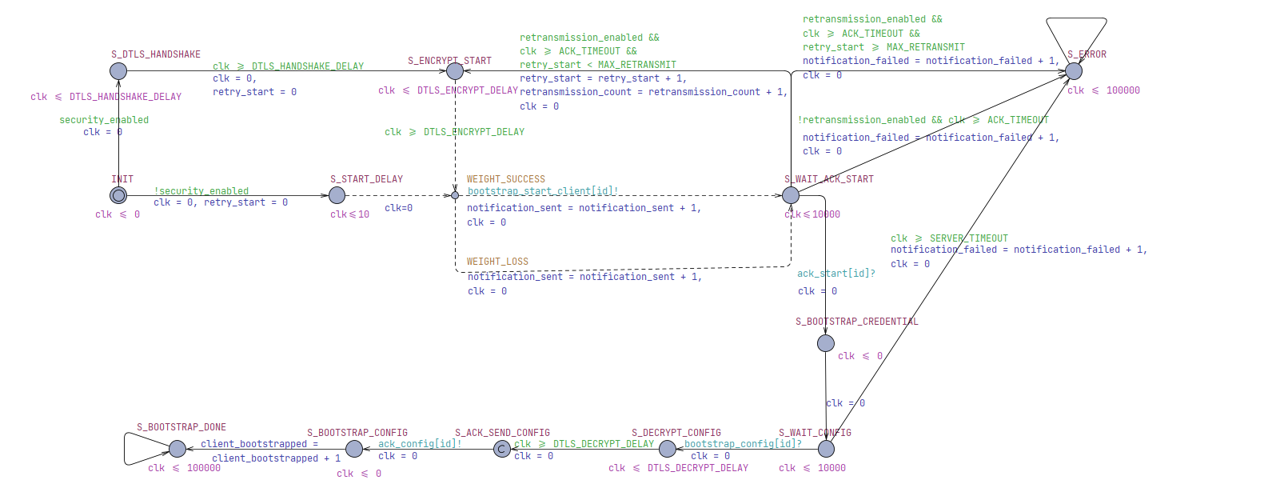
\includegraphics[width=\textwidth]{figs/bootstrapclientsmc.png}
	\caption{Bootstrap Client Model with Packet Loss and Retransmission Mechanism.}
	\label{smcbootstrap}
\end{figure}

For Registration, the model is simpler because only the initial \texttt{register\_start} is a CON message; the response \texttt{register\_complete} is a NON message. Hence, only the client performs retransmissions, while the server sends the response without waiting for an ACK.

\subsubsection{Verification Results}
The same three experimental configurations (A: no security, no retransmission; B: DTLS only; C: DTLS + retransmission) are applied. The parameters are identical to those used in Observation, except that the simulation time bound is reduced to $5000ms$ because the interaction is shorter. The verified properties are the success probability (whether the client reaches the final registered state) and, for configuration C, the number of retransmissions.

The results (Table ~\ref{tab:bootstrap-registration-perf-results}) show that DTLS introduces a slight decrease in success probability (from $0.986$ to $0.982$), while adding retransmission brings the success probability to 1 for both interfaces, confirming the effectiveness of CoAP‑style retransmission in lossy environments.

\begin{table}[htbp]
\centering
\caption{Performance evaluation results for the bootstrap and registration interfaces. Values are given as estimate ± half‑width of the $95\%$ confidence interval.}
\label{tab:bootstrap-registration-perf-results}
\begin{tabular}{llccc}
\toprule
\textbf{Interface} & \textbf{Configuration} & \textbf{Success Probability} & \textbf{Throughput (max notifications)} & \textbf{Retransmissions (max)} \\
\midrule
\multirow{3}{*}{Bootstrap}
 & A & 0.986 ± 0.014  & – & – \\
 & B & 0.982 ± 0.014  & – & – \\
 & C & 1.000 ± 0.000  & – & 0.005 ± 0.010 \\
\midrule
\multirow{3}{*}{Registration}
 & A & 0.986 ± 0.014  & – & – \\
 & B & 0.982 ± 0.014  & – & – \\
 & C & 1.000 ± 0.000  & – & 0.005 ± 0.010 \\
\bottomrule
\end{tabular}
\end{table}

From the above statistics, we can conclude that DTLS introduces a small decrease in success probability (from 0.986 to 0.982) due to the additional handshake and encryption delays, but the difference is not statistically significant given the confidence intervals.
With retransmission, the success probability becomes 1 for both interfaces, confirming that the CoAP‑style retransmission mechanism effectively recovers from packet loss.
The very low retransmission count (0.005) again reflects the low baseline loss probability.

\subsection{Summary of Performance Layer}
The probabilistic models demonstrate that LwM2M can achieve high reliability even under realistic network conditions. The introduction of security mechanisms (DTLS and OSCORE) incurs a moderate performance penalty (about $7\%$ lower throughput for observation, and a slight reduction in success probability for bootstrap and registration). However, when combined with the CoAP retransmission mechanism, the system can completely compensate for packet loss, achieving near‑perfect reliability. These results provide a quantitative basis for choosing appropriate security and reliability configurations in industrial deployments.

\section{Conclusion and Future Work}
In this paper, we have presented a three‑layer formal framework for the LwM2M protocol in industrial IoT scenarios. Layer I builds deterministic UPPAAL models for Bootstrap, Registration, and Observation, verifying functional correctness (reachability, deadlock freedom). Layer II integrates attacker automata (MITM, eavesdropping, fake BS, replay, DoS, tampering), confirming the feasibility of all modeled attacks and exposing the lack of integrity and freshness. Layer III uses UPPAAL SMC to evaluate probabilistic packet loss ($0.5\%$), CoAP retransmissions, and OSCORE/DTLS overhead. Results show that security mechanisms incur a moderate penalty ($\approx7\%$ throughput drop), but combined with retransmissions they achieve near‑perfect reliability. All models are available as supplementary material.

For future work, we plan to extend the security model with more sophisticated attackers, such as those exploiting timing channels or physical‑layer vulnerabilities (e.g., jamming, side‑channel leakage). This would allow us to assess the resilience of LwM2M against advanced persistent threats that go beyond simple message tampering or replay. Second, we intend to apply our three‑layer verification framework to other widely used industrial IoT protocols, such as MQTT and OPC UA. By conducting a horizontal comparative study, valuable guidance can be provided for selecting the most suitable protocol for specific manufacturing scenarios, balancing security, reliability, and efficiency.



% \textbf{Acknowledgments}
\section*{Acknowledgments}
This work was partially supported by the National Key Research and Development Program of China (No. 2022YFB3305102).

\printcredits

%% Loading bibliography style file
\bibliographystyle{model1-num-names}
% \bibliographystyle{cas-model2-names}

% Loading bibliography database
\bibliography{cas-refs}


% \bio{figs/pic1}
% Sini Chen is currently a Ph.D student in Shanghai Key Laboratory of Trustworthy Computing, East China Normal University, Shanghai. She received her B.S. degree in software engineering in East China Normal University in 2021. Her research interests include process algebra, program semantics, object-oriented systems and LLM-assisted verification.
% \endbio
% \vspace{2cm}
% \bio{figs/pic2}
% Ran Li is currently a lecturer with the School of Computer Science & School of Software, Nanjing University of Information Science and Technology. She received the B.S. (2018) and Ph.D. (2023) in software engineering from East China Normal University, China. Her research interests include formal semantics, formal verification, and process algebra.
% \endbio
% \vspace{2cm}
% \bio{figs/pic3}
% Zihan Tang is currently an M.S. student in Shanghai Key Laboratory of Trustworthy Computing, East China Normal University, Shanghai. He received the B.S. degree in software engineering from Donghua University, Shanghai, China, in 2025. His research interests include formal methods, process algebra and its applications, probabilistic model checking, protocol analysis and LLM-assisted verification.
% \endbio
% \vspace{2cm}
% \bio{figs/pic4}
% Huibiao Zhu is currently a professor in East China Normal University, Shanghai. He earned his Ph.D.
% degree in formal methods from London South Bank University, London, in 2005. During these
% years, he has studied various semantics and their linking theories for Verilog, SystemC, web ser
% vices and probability system. He was the Chinese PI of the Sino-Danish Basic Research Center
% IDEA4CPS.
% \endbio

% \bio{figs/pic1}
% Author biography with author photo.
% \endbio

\end{document}
